\chapter{Зависимость насыщающего вейбелевскую неустойчивость магнитного поля от вида распределения частиц по скоростям}
\newcommand{\PunctumKappa}{-}
\label{ch:ch5}
\section{Введение}\label{ch:ch5/sec1}
Неравновесной плазме, частицы которой испытали стохастическое ускорение под действием того или иного широкополосного электромагнитного излучения свойственно наличие наличие надтеплового {\glqq}хвоста{\grqq} в энергетическом распределении частиц~\cite{Maksimovic2005, Vasyliunas1968,Lazar2022}.
В этой связи актуальны задачи лабораторной астрофизики с лазерной плазмой~\cite{Romanov2004, Thaury2010, Silva2020, Shukla2020, Zhang2020}, получаемой абляцией различных мишеней фемтосекундными импульсами петаваттных лазеров, и задачи физики солнечного (звездного) ветра, начиная с корональных областей его происхождения и кончая границами между магнитными облаками в нем или областями его взаимодействия с магнитосферами планет~\cite{Baumjohann2012, Dudik2017, Livadiotis2017,Marsch2006,Yoon2017,Echim2010}.
Для обоих указанных классов задач имеется непосредственная возможность получать информацию как о распределении частиц по энергии, так и об анизотропии распределения частиц по скоростям. 
Наблюдаемый надтепловой {\glqq}хвост{\grqq}, свойственный также различным каппа{\PunctumKappa}распределениям, делает последние удобными для использования в численном моделировании процессов развития вейбелевской неустойчивости и генерации долгоживущей квазимагнитостатической турбулентности. 

В рамках обычно рассматриваемой начальной пространственно однородной задачи неоднократно проверялось, что возникающая с уровня шумов турбулентность и среднеквадратичная величина связанного с ней магнитного поля в существенной мере зависят от начальной анизотропии распределения частиц~(см. раздел \ref{sec:ch2/sec2} настоящей работы, а также \cite{Lemons1979, Kato2005, Borodachev2010,Davidson1972,Ruyer2015,Lazar2022}).
Тем не менее эта зависимость остается мало изученной, особенно если учесть чувствительность выводов о развитии вейбелевской неустойчивости к виду распределения частиц по энергиям~\cite{Lazar2010,Silva2021}. 

В данной главе, как и в главах \ref{ch:ch1}-\ref{ch:ch3}, для определенности эффективная температура частиц считается наибольшей вдоль оси $y$. 
Тогда если бы в трехмерном случае функция распределения (ФР) частиц обладала аксиальной симметрией по отношению к скоростям в плоскости $x,z$, то неустойчивость развивалась только для волновых возмущений необыкновенного типа и приводила к ТМ-вейбелевской турбулентности~\cite{Kalman1968, Vagin2014}.
Имея в виду аналогичную ситуацию для рассматриваемых ниже двумерных расчетов, будем считать ФР симметричной по проекции скорости частиц на ось $x$, т.\,е. не зависящей от знака этой проекции. 
Для рассматриваемых ТМ-возмущений в данном случае волновые векторы гармоник электромагнитного поля и соответствующих гармоник анизотропной ФР энергонесущих частиц (пусть электронов), как и вектор электрического поля, лежат в плоскости $x,y$, а вектор магнитного поля ортогонален этой плоскости, т.\,е. параллелен оси $z$ (рис.~\ref{fig:GeomIsolines}б). 
Как видно из разделов \ref{sec:ch2/sec2} и \ref{ch:ch4/sec5}, неустойчивость насыщается, т.\,е. прекращается рост среднеквадратичного магнитного поля, тогда, когда оно в достаточной мере выравнивает средние значения продольной ($T_{\|}$, вдоль оси $y$) и поперечной ($T_\perp $, вдоль оси $x$) эффективных температур. 
При этом присутствие этого поля, его пространственная неоднородность и понизившийся и тоже неоднородный уровень анизотропии $A=T_{\|} / T_{\perp} - 1$ исключают экспоненциальное нарастание каких-либо возмущений, в том числе крупномасштабных, хотя слабонелинейная перестройка пространственного спектра турбулентности в длинноволновую сторону продолжается и далее (см. главы \ref{ch:ch2} и \ref{ch:ch2} настоящей работы, а также \cite{Kuznetsov2022,Kuznetsov2023,Kocharovsky2016,Zhou2022, Borodachev2016_Radiofiz,Dieckmann2009,Romanov2004}).

\begin{figure}[h]
\begin{minipage}[c]{0.5\linewidth}
    \includegraphics[width=1\linewidth]{part5/levels.eps}
\end{minipage}
\begin{minipage}[c]{0.5\linewidth}
    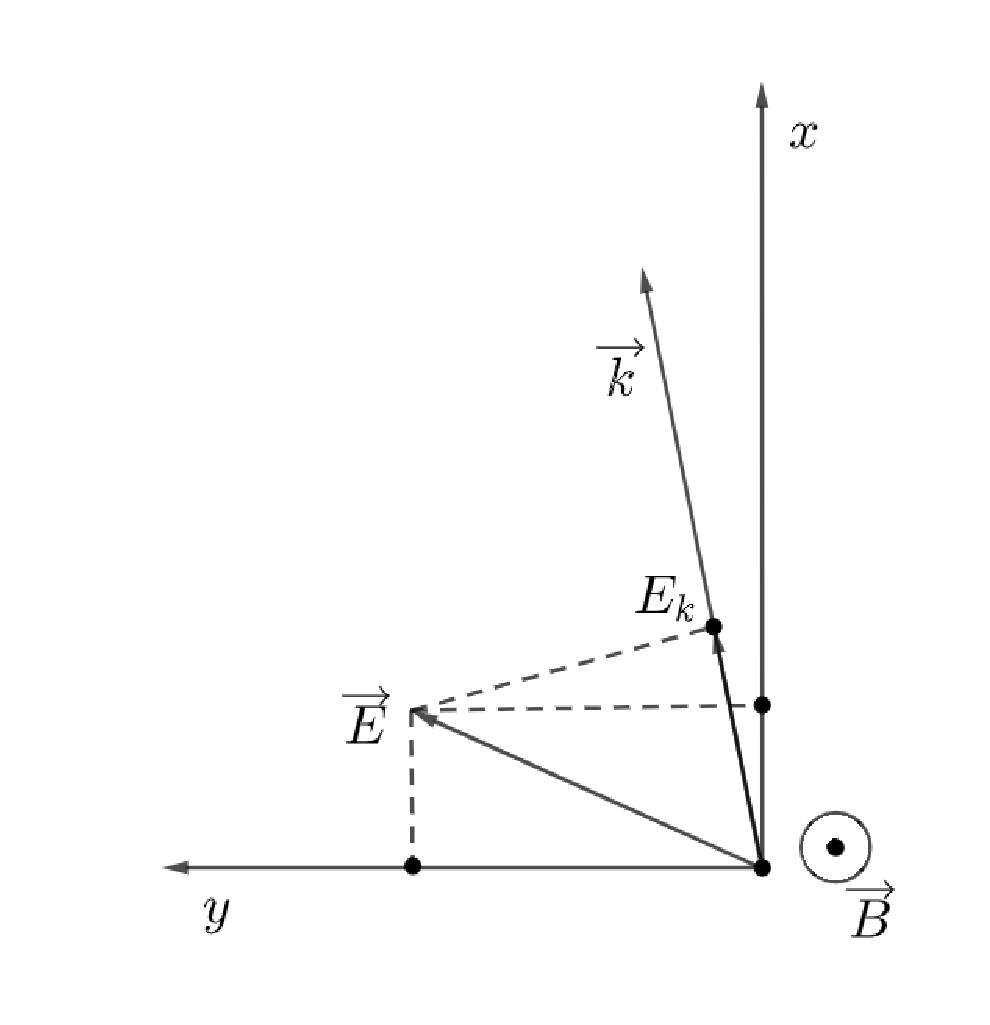
\includegraphics[width=1\linewidth]{part5/new_image.eps}
\end{minipage}
\captionstyle{normal}
    \caption{
    а)~Линии уровня $0.001$, $0.1$ и $0.9$ от максимального значения для бимаксвелловской (сплошная кривая), бикаппа{\PunctumKappa} (штриховая) и продакт-бикаппа{\PunctumKappa} (штрихпунктир) функций распределения электронов по нормированным скоростям $\beta_x$ и $\beta_y$ при $\kappa=2$, поперечной (вдоль оси~$x$) тепловой скорости $\beta_\perp=0.1$ и параметре анизотропии $A = 1$. 
    б)~Взаимное расположение волнового вектора $\vec{k}$, лежащего в плоскости $x,y$, и векторов магнитного $\vec{B}$ и электрического $\vec{E}$ полей в отдельной пространственной гармонике ТМ-вейбелевской турбулентности.
    }
\label{fig:GeomIsolines}
\end{figure}

Предположим, что в начальный момент времени нормированная на единицу функция распределения имеет вид бикаппа{\PunctumKappa}распределения с $\kappa >  1$, 
\begin{equation}
\label{eq:kappa}
    \Psi(\vec{\beta})=\dfrac{1}{\pi\theta_{\perp}\theta_{\|} } \left(1+\dfrac{\beta_x^2}{\kappa\theta_{\perp}^2}+\dfrac{\beta_y^2}{\kappa\theta_{\|}^2}\right)^{-\kappa-1} ,
\end{equation}
либо продакт-бикаппа{\PunctumKappa}распределения с $\kappa > 1/2$, 
\begin{equation}
\label{productkappa}
\Psi(\vec{\beta}) = \dfrac{\Gamma^2(\kappa+1)}{\Gamma^2(\kappa+0.5)} \: \dfrac{1}{\pi\kappa\theta_{\perp}\theta_{\|}}\left(1+\dfrac{\beta_x^2}{\kappa\theta_{\perp}^2}\right)^{-\kappa-1} \!\left(1+\dfrac{\beta_y^2}{\kappa\theta_{\|}^2}\right)^{-\kappa-1};
\end{equation}
см.~\cite{Lazar2010, Livadiotis2017, Livadiotis2021,Pierrard2010}. 
Выше введены характерные скорости $\theta_{\perp,\|}=\beta_{\perp,\|}\left(1-1/\kappa\right)^{1/2}$ для бикаппа{\PunctumKappa}распределения и $\theta_{\perp,\|}=\beta_{\perp,\|}\left(1-1/(2\kappa)\right)^{1/2}$ для продакт-бикаппа{\PunctumKappa}распределения с использованием эффективных тепловых скоростей $\beta_{\perp,\|}$ вдоль осей $x$ и $y$ соответственно, так что параметр анизотропии
\begin{equation}
A={\beta^2_{\|}}/{\beta^2_{\perp}}-1={\theta^2_{\|}}/{\theta^2_{\perp}}-1.
\end{equation}
В пределе $\kappa \rightarrow \infty$ распределения (\ref{eq:kappa}), (\ref{productkappa}) сводятся к бимаксвеллловскому (\ref{bimax}).
Его характерные сечения, как и сечения распределений (\ref{eq:kappa}), (\ref{productkappa}) при $\kappa=2$, представлены на рис.~\ref{fig:GeomIsolines}а для параметра анизотропии $A=1$. 
На рис.~\ref{fig:GeomIsolines}б для поставленной задачи показано расположение векторов электрического $\vec{E}$ и магнитного $\vec{B}$ полей рассматриваемых однородных гармоник необыкновенного типа $\exp(-i\vec{k}\vec{r})$ с волновым вектором $\vec{k}$, проекция на который электрического поля в общем случае не равна нулю: $E_k\neq0$.

С целью анализа насыщения развивающейся ТМ-вейбелевской неустойчивости используем ранее описанный квазилинейный подход к описанию квазимагнитостатической турбулентности, использующий разложение по пространственным гармоникам решения уравнений Власова~-- Максвелла с шумоподобным начальным возмущением магнитного поля, обладающим примерно равномерным спектром в области неустойчивых волновых чисел. 
При этом наличие большого числа однотипных гармоник, обладающих случайными фазами и достаточно плотно заполняющих значимую область волновых векторов, обеспечивает гладкую форму и плавность изменения ФР, исключая сколько-нибудь значительные эффекты когерентной интерференции и допуская неадекватный вид ФР, например отрицательные ее значения, только при скоростях много больше эффективных тепловых, т.\,е. для очень малой, несущественной фракции электронов.

Как и в главе \ref{ch:ch3}, в рассматриваемомо случае двумерно-неоднородной задачи с большим числом $m \cdot s$ неколлинеарных производящих гармоник
$\{ (k_{1}; k_{1}),\, (k_{1}; k_{2}),...,\, (k_{2}; k_{1}),...\, (k_{m}; k_{s}) \}$ (их компоненты состоят из $m$ проекций $\vec{k}\vec{x_0}$ и $s$ проекций $\vec{k}\vec{y_0}$), расположенных часто и перекрывающих всю существенную область волновых векторов неустойчивости,
магнитное поле имеет вид суммы по целочисленному векторному индексу $\vec{n}=(n_x,n_y)$:
$B(t,x,y)= \mathrm{Re} \, \sum^{m}_{n_x=1}\sum_{n_y=1}^sB_{k_{\vec{n}}}(t)\exp(- ik_{n_{x}}x - ik_{n_{y}}y)$.
Аналогичный вид имеет каждая из двух кратных гармоник-возмущений ФР, т.\,е. компонент $\delta f_1(t,x,y)$ и $\delta f_2(t,x,y)$, разложенных на комплексные гармоники ${f_1}_{k_{\vec{n}}}(t)$ и ${f_2}_{k_{\vec{n}}}(t)$ соответственно; нулевая (действительная) гармоника $f_0(t)=\delta f_0(t)$ зависит только от вектора скорости и дает поправку к ФР, усредненную по плоскости $x,y$. 

\begin{equation}
\label{eq14_ch5}
    \dfrac{\partial \psi_0}{\partial \tau} 
    + \sum\limits^{m,s}_{n_x,n_y=1}\left( \hat \Phi(b_{K_{\vec{n}}},\psi_{K_{\vec{n}}}^*) 
    + \hat \Phi^*(b_{K_{\vec{n}}}^*,\psi_{K_{\vec{n}}}) \right)=0,
\end{equation}
\begin{equation}
    \dfrac{\partial \psi_{K_{\vec{n}}}}{\partial \tau}+iK_{n_x}\beta_x\psi_{K_{\vec{n}}}+iK_{n_y}\beta_y\psi_{K_{\vec{n}}}+2\hat \Phi(b_{K_{\vec{n}}},\Psi(\vec{v})+\psi_0)+\hat \Phi^*(b_{K_{\vec{n}}}^*,\psi_{2K_{\vec{n}}})=0,
\end{equation}
\begin{equation}
\label{eq16_ch5}
    \dfrac{\partial \psi_{2K_{\vec{n}}}}{\partial \tau}+2iK_{n_x}\beta_x\psi_{2K_{\vec{n}}}+2iK_{n_y}\beta_y\psi_{2K_{\vec{n}}}+\hat \Phi(b_{K_{\vec{n}}},\psi_{K_{\vec{n}}})=0,
\end{equation}
\begin{equation}
    \dfrac{\partial b_{K_{\vec{n}}}}{\partial \tau}=-ie_{y{K_{\vec{n}}}}K_{n_x}+ie_{x{K_{\vec{n}}}}K_{n_y},
\end{equation}
\begin{equation}
    \dfrac{\partial e_{x{K_{\vec{n}}}}}{\partial \tau}=ib_{K_{\vec{n}}}K_{n_y}-\beta_{\|}^{-1}\iint\limits^{+\infty}_{-\infty}\beta_x\psi_{K_{\vec{n}}}(\tau,\beta_x,\beta_y)d\beta_xd\beta_y,
\end{equation}
\begin{equation}
\label{eq19_ch5}
    \dfrac{\partial e_{y{K_{\vec{n}}}}}{\partial \tau}=-ib_{K_{\vec{n}}}K_{n_x}+\beta_{\|}^{-1}{\iint\limits^{+\infty}_{-\infty}\beta_y\psi_{K_{\vec{n}}}(\tau,\beta_x,\beta_y)d\beta_xd\beta_y} .
\end{equation}
Здесь использованы безразмерные время и волновое число, 
\begin{equation*}
    \tau=\wpl t, \
    K=\dfrac{kc}{\wpl}; \ 
    \wpl^2=\dfrac{4\pi Ne^2}{\me},
\end{equation*}
а также нормированные (комплексные) гармоники магнитного поля и ФР: 
\begin{equation}
\label{eq19plus1_ch5}
    b_{K_{\vec{n}}}=\dfrac{B_{K_{\vec{n}}}}{\sqrt{8\pi N T_{\|}}},\
    T_{\|}=\dfrac{m_ec^2\beta_{\|}^2}{2};\
    \psi_{\ell\cdot K_{\vec{n}}}=\dfrac{c^2f_{\ell\cdot K_{\vec{n}}}}{N},\ 
    \ell=0,\,1,\,2.  
\end{equation}
Комплексные компоненты электрического поля $e_{x{K_{\vec{n}}}}$ и $e_{y{K_{\vec{n}}}}$ (см. рис.~\ref{fig:GeomIsolines}б) нормированы так же, как магнитное поле $b_{K_{\vec{n}}}$. 
Для удобства вновь введен оператор:
\begin{equation}
\label{eq:operator_ch5}
    \hat \Phi(b_{K_n},e_{x{K_{\vec{n}}}},e_{y{K_{\vec{n}}}},\psi(\vec{\beta}))=\dfrac{e_{y{K_{\vec{n}}}}}{2}\dfrac{\partial \psi(\vec{\beta})}{\partial \beta_y}+\dfrac{e_{x{K_{\vec{n}}}}}{2}\dfrac{\partial \psi(\vec{\beta})}{\partial \beta_x}-\dfrac{b_{K_n}}{2} \left(\beta_x\dfrac{\partial \psi(\vec{\beta})}{\partial \beta_y}-\beta_y\dfrac{\partial \psi(\vec{\beta})}{\partial \beta_x}\right).
\end{equation}

Представленная система интегро-дифференциальных уравнений (\ref{eq14_ch5})--(\ref{eq19_ch5}) с оператором (\ref{eq:operator_ch5}) решалась, как и в предыдущих случаях, стандартным методом Стёрмера~-- Верле (Leapfrog)~\cite{Birdsall2018}. 

Шаг по времени $d\tau$ составлял малую величину $d\tau\sim 0.05$--$0.5$ в сравнении с наименьшим временным масштабом рассматриваемой обезразмеренной системы уравнений, который определяется собственными длинами волн магнитного поля и тока ($\sim \! {\pi}/{K}$) и имеет порядок единицы. 
Расчетная сетка для нормированных скоростей $\beta_x$, $\beta_y$ как переменных трех компонент (\ref{eq14_ch5})--(\ref{eq16_ch5})  анизотропной ФР, разложенных по производящим гармоникам, выбиралась анизотропной с соответствующими шагами $d\beta_x\sim{\beta_{\perp}}/{15}$ и $d\beta_y\sim{\beta_{\|}}/{15}={\beta_{\perp}\sqrt{1+A}}/{15}$. 
Количество производящих пространственных гармоник $m\cdot s$ в типичных расчетах составляло несколько тысяч и выбиралось из условия независимости (с точностью до нескольких процентов) вычисляемого магнитного поля насыщения неустойчивости от дальнейшего увеличения чисел $m$ и $s$, что обычно имело место начиная с чисел $\sim\! 100$ и $\sim\! 30$ соответственно. 

\section{Особенности насыщения неустойчивости для бикаппа-распределения электронов}
\label{ch:ch5/sec2}
Основные результаты численного моделирования вейбелевской неустойчивости в двумерной задаче суммированы на рис.~\ref{fig:kappa_sat} и \ref{fig:pr_kappa_sat} в представительном интервале параметров начальной анизотропии $0.1\leq A \leq 20$. 
Как и ожидалось, максимальная величина среднего квадрата нормированного магнитного поля $b_{sat}^2 = {({8\pi N T_{\|}})^{-1}} \sum_{\vec{n}} {|B_{K_{\vec{n}}}|^{2}} $, достигаемая в ходе ТМ-неустойчивости, растет с увеличением анизотропии $A$. 
При малых значениях $A < 1$ рост оказывается довольно быстрым и зависящим от энергетического распределения электронов. 
Он теряет эту зависимость и замедляется при $A > 1$, останавливаясь на уровне немного выше 10\% в пределе $A \gg 1$. 
О последнем свидетельствуют также контрольные расчеты, выполненные для бимаксвелловского распределения с $A = 1$, $10$, $30$ с использованием кода EPOCH~\cite{Arber2015}, т.\,е. методом частиц в ячейках (PIC). 
Результаты применения обоих подходов совпадают с точностью порядка 10\%-30\% и подтверждают известную оценку насыщающего магнитного поля, в которой обратный гирорадиус и гирочастота типичных частиц по порядку величины сравниваются соответственно с волновым числом и инкрементом наиболее сильно выросших гармоник поля~\cite{Borodachev2016_Radiofiz, Nechaev2019_Radiophys, Garasev2022_JPP}, что было проверено для всех проведенных расчетов. 
Предшествующие аналогичные расчеты для отдельных значений параметра анизотропии $A = 24$ и $A = 99$ представлены в~\cite{Morse1971, Stockem2009}. 

\begin{figure}[h]
\includegraphics[width=0.5\linewidth]{part5/14132.eps}
\captionstyle{normal}
\centering
\caption{Зависимость среднего квадрата нормированного насыщающего магнитного поля (см. (\ref{eq19plus1}))  от параметра анизотропии $A$ для бикаппа{\PunctumKappa}распределения (\ref{eq:kappa}) при $\beta_\perp=0.1$ и различных значениях параметра каппа:  $\kappa=2$~--- штрихи, $\kappa=\infty$~--- сплошная кривая (бимаксвелловское распределение). В последнем случае крестиками показаны три контрольные точки, рассчитанные в рамках 2D3V кода EPOCH методом частиц в ячейках.}
\label{fig:kappa_sat}
\end{figure}

С использованием метода частиц в ячейках трехмерные расчеты подобной зависимости ни для какой геометрии еще не проводились, а детальные двумерные расчеты известны лишь для аксиально симметричного бимаксвелловского распределения частиц с осью наибольшей температуры, ортогональной плоскости расчета, для параметров анизотропии $A \sim 0.1$--\,$50$~(см. в этой связи \cite{Kato2005, Borodachev2010}, а также раздел \ref{sec:ch2/sec2} настоящей работы).
Примеры насыщения аналогичной неустойчивости, называемой филаментационной, в случае двух встречных пучков частиц см. в~\cite{Dieckmann2009,Ruyer2015}. 
В вышеуказанных работах, посвященных вейбелевской ТЕМ-неустойчивости насыщающее поле отличается от представленных на рис.~\ref{fig:kappa_sat}, \ref{fig:pr_kappa_sat} значений на величину $\sim \! 10\%$\,--\,50\%, что связано с учетом только ортогональных оси анизотропии волновых векторов, приводящим к двумерно изотропной турбулентности. 
В данной же главе рассматривается случай, когда допустимы любые углы наклона волнового вектора к оси анизотропии $y$, лежащей в плоскости расчета, так что спектр турбулентности оказывается существенно анизотропным и для насыщения неустойчивости магнитное поле должно нарасти до немного другой величины.
Как уже отмечалось для бимаксвелловского начального распределения частиц по скоростям (см. раздел \ref{sec:ch2/sec2}), одномерные расчеты для малых параметров анизотропии $A \ll 1$, как и приближенная квазилинейная теория (ср.~\cite{Pokhotelov2011, Dieckmann2009, Ruyer2015}), многократно занижают насыщающее магнитное поле и неприменимы для оценки его реальных значений в двумерной и трехмерной постановках задачи. 

Недостатком метода частиц в ячейках, кроме больших затрат вычислительных ресурсов, является высокий уровень численных шумов ФР частиц, вообще говоря, спектрально неравномерный. 
Это обстоятельство понижает точность и ограничивает возможность проведения корректных расчетов, особенно при малых параметрах анизотропии $A \ll 1$, когда неустойчивость развиваются настолько медленно, что скорость изотропизации частиц на шумовой компоненте электромагнитного поля становится сравнимой с инкрементом вейбелевской неустойчивости. 
Такого недостатка нет в развитом методе возмущений на основе пространственных гармоник, где шумы легко контролируются и могут быть адекватно заданы выбором подходящего спектра начального магнитного поля. 

Согласно проведенным расчетам с использованием уравнений (\ref{eq14_ch5})--(\ref{eq:operator_ch5}), для бимаксвелловского распределения средний квадрат насыщающего магнитного поля ТМ-вейбелевской неустойчивости $b_{sat}^2$ лишь немного, не более чем на 30\% превышает его значение для бикаппа{\PunctumKappa}распределений при $\kappa\geq2$; см. рис. \ref{fig:kappa_sat}. 
Более того, для этих бикаппа- и бимаксвелловского распределений характерные волновые числа $k_x$, отвечающие максимуму спектра развивающейся турбулентности в ортогональном оси анизотропии направлении $\vec{x_0}$, и характерные ширины этого спектра вдоль осей $x$ и $y$ оказались почти идентичными как на линейной стадии неустойчивости, так и в течении ее долговременной квазилинейной эволюции. 
Близость значений насыщающего магнитного поля для указанных распределений (\ref{eq:kappa}) и (\ref{bimax}) согласуется с близостью инкрементов обусловленных ими вейбелевских неустойчивостей (рис. \ref{fig:kappa_inkr}), найденных из численных расчетов среднеквадратичного магнитного поля на этапе его экспоненциального роста задолго до момента насыщения. 
Эти инкременты лишь немного меньше максимальных инкрементов, вычисленных из соответствующих дисперсионных уравнений (о последних см., например,~\cite{Mikhailovsky1971, Lazar2006, Vagin2014, Kocharovsky2016,Ruyer2015,Silva2021}). 

\begin{figure}[h]
\includegraphics[width=0.5\linewidth]{part5/kappa_inkr.eps}
\captionstyle{normal}
\centering
\caption{Зависимость инкремента $\gamma$ (нормированного на плазменную частоту $\wpl$) среднеквадратичного магнитного поля от параметра анизотропии $A$ для бикаппа{\PunctumKappa}распределения (\ref{eq:kappa}) при $\beta_\perp=0.1$ и различных значениях параметра каппа: $\kappa=2$~--- штрихи, $\kappa=\infty$~--- сплошная кривая (бимаксвелловское распределение).}
\label{fig:kappa_inkr}
\end{figure}

Полученный результат согласуется также с практически одинаковой формой деформации указанных ФР электронов к моменту насыщения неустойчивости, о чем можно судить, прежде всего, из найденных в наших расчетах пространственно однородных поправок $\delta f_0(v_x, v_y)$, т.\,е. $\delta \psi_0(\beta_x, \beta_y)$. 
Соответствующая деформация ФР вызвана совокупным действием всех гармоник квазимагнитостатической турбулентности и в свою очередь определяет квазилинейную эволюцию каждой из этих гармоник, непосредственно не взаимодействующих между собой: их начальное нарастание, длительное существование с медленным изменением амплитуды и последующее неизбежное затухание. 

\section{Особенности насыщения неустойчивости для продакт-бикаппа{\PunctumKappa}распределения электронов}
\label{ch:ch5/sec3}

\begin{figure}[h]
\includegraphics[width=0.5\linewidth]{part5/1370_fin.eps}
\captionstyle{normal}
\centering
\caption{Зависимость среднего квадрата нормированного насыщающего магнитного поля (см. (\ref{eq19plus1}))  от параметра анизотропии $A$ для продакт-бикаппа{\PunctumKappa}распределения (\ref{productkappa}) при $\beta_\perp=0.1$ и различных значениях параметра каппа: $\kappa=1$~--- штрихпунктир, $\kappa=2$~--- штрихи, $\kappa=4$~--- пунктир, $\kappa=\infty$~--- сплошная кривая (бимаксвелловское распределение).}
\label{fig:pr_kappa_sat}
\end{figure}

Детализируем сделанные выше общие утверждения применительно к продакт-бикаппа{\PunctumKappa}распределению (\ref{productkappa}), для которого обнаруживается существенное влияние величины $\kappa$ на исследуемую зависимость насыщающего поля от начальной анизотропии ФР, особенно в области ее малых величин $A<0.8$ согласно рис.~\ref{fig:pr_kappa_sat}. 
Монотонные зависимости среднего квадрата насыщающего магнитного поля от параметра анизотропии $A$ для различных величин $\kappa$ имеют разный наклон и пересекаются в одной точке $A=0.8$. 
При $A \sim 0.1$ эти зависимости приближенно являются степенными с показателями, которые примерно равны 2/5, 2/3, 1, 2 для $\kappa =$ 1, 2, 4, $\infty$ соответственно (и могут оказаться меньше при $A < 0.1$).  

Ниже точки $A=0.8$ квадрат насыщающего магнитного поля $b_{sat}^2$ значительно падает с ростом величины $\kappa$, достигая минимального значения при $\kappa \rightarrow \infty$, т.\,е. для бимаксвелловского распределения. 
Напротив, выше указанной точки $A=0.8$ величина $b_{sat}^2$ растет с ростом $\kappa$, хотя и не столь значительно, поскольку ее максимальное значение для величины $\kappa$ вблизи 1 составляет несколько процентов и всего в пару раз меньше предельно достижимого значения квадрата магнитного поля $b_{sat}^2$, реализующегося для бимаксвелловского распределения и немного превышающего 10\%. 

Для продакт-бикаппа{\PunctumKappa}распределений в отличие от бикаппа{\PunctumKappa}распределений величина $\kappa$ гораздо значительнее влияет на нелинейную эволюцию как характерного волнового числа $k_x$, отвечающего максимуму спектра турбулентности и направленного в ортогональном оси анизотропии направлении $\vec{x_0}$, так и характерных ширин турбулентного спектра вдоль осей $x$ и $y$. С ростом величины $\kappa$ уширение спектра вдоль оси анизотропии ФР увеличивается, тогда как ширина спектра поперек этой оси уменьшается одновременно с уменьшением указанной проекции $k_x$ волнового вектора максимума турбулентного спектра.
Подобное уменьшение наиболее существенно на начальной нелинейной стадии эволюции спектра (и становится довольно малым на поздней стадии, которой мы не интересуемся в настоящей работе).

Сделанное наблюдение согласуется с уменьшением при росте $\kappa$ инкремента нарастания магнитного поля (рис.~\ref{fig:pr_kappa_inkr}), вычисленного на линейной стадии задолго до насыщения неустойчивости и примерно равного максимальному инкременту, получающемуся из соответствующего дисперсионного уравнения (см.~о~нем~\cite{Mikhailovsky1971, Lazar2006, Vagin2014, Kocharovsky2016,Ruyer2015,Silva2021}). Уменьшение инкремента с увеличением $\kappa$ от 1 до $\infty$ значительно лишь для небольшой начальной анизотропии $A \lesssim 1$: для $A=1$ инкремент уменьшается примерно вдвое, а для $A=0.1$~--- в 20 раз. Заметим, что в последнем случае почти в 20 раз уменьшается и квадрат насыщающего магнитного поля $b_{sat}^2$ (рис.~\ref{fig:pr_kappa_sat}). Вместе с тем это поле слабо зависит от величины $\kappa$ при большой начальной анизотропии $A \gg 1$.
\begin{figure}[h]
\includegraphics[width=0.5\linewidth]{part5/1372_fin.eps}
\captionstyle{normal}
\centering
\caption{Зависимость инкремента $\gamma$ (нормированного на плазменную частоту $\wpl$) среднеквадратичного магнитного поля от параметра анизотропии $A$ для продакт-бикаппа{\PunctumKappa}распределения (\ref{productkappa}) при $\beta_\perp=0.1$ и различных значениях параметра каппа: $\kappa=1$~--- штрихпунктир, $\kappa=2$~--- штрихи, $\kappa=4$~--- пунктир, $\kappa=\infty$~--- сплошная кривая (бимаксвелловское распределение).}
\label{fig:pr_kappa_inkr}
\end{figure}


Выведенная в настоящей работе система приближенных уравнений (\ref{eq14_ch5})--(\ref{eq19_ch5}), (\ref{eq:operator_ch5}) для ТМ-гармоник турбулентности позволяет исследовать насыщение вейбелевской неустойчивости и ее дальнейшую нелинейную эволюцию при малых величинах параметра анизотропии, включая область $A \lesssim 0.01$ (которая вряд ли легко доступна расчетам методом частиц в ячейках из-за неизбежных для него численных шумов). 
Подобная близость к порогу неустойчивости характерна для многих физических ситуаций, и особенности обсуждаемого эффекта насыщения роста ТМ-вейбелевской турбулентности в этих условиях заслуживают специального исследования.

В этом отношении актуальны, например, задачи лабораторной астрофизики с лазерной плазмой~\cite{Romanov2004, Thaury2010, Silva2020, Shukla2020, Zhang2020}, получаемой абляцией различных мишеней фемтосекундными импульсами петаваттных лазеров, и задачи физики солнечного (звездного) ветра, начиная с корональных областей его происхождения и кончая границами между магнитными облаками в нем или областями его взаимодействия с магнитосферами планет~\cite{Baumjohann2012, Dudik2017, Livadiotis2017,Marsch2006,Yoon2017,Echim2010}. 
Для обоих указанных классов задач имеется непосредственная возможность получать информацию как о распределении частиц по энергии, так и об анизотропии распределения частиц по скоростям. 
Наблюдаемое наличие надтеплового {\glqq}хвоста{\grqq} в энергетическом распределении частиц~\cite{Maksimovic2005, Vasyliunas1968,Lazar2022}, свойственное различным каппа{\PunctumKappa}распределениям, делает последние удобными для использования в численном моделировании процессов развития вейбелевской неустойчивости и генерации долгоживущей квазимагнитостатической турбулентности. 

Выполненное в настоящей главе исследование зависимостей насыщающего среднеквадратичного магнитного поля от параметров каппа $\kappa$ и анизотропии $A$ представляется важным для оценки влияния такого рода турбулентности на ряд наблюдаемых явлений в лазерной и космической плазме. 
В частности, важными представляются найденные конкретные зависимости уровня насыщения вейбелевской турбулентности от параметра анизотропии, которые для одних ФР (например, бикаппа{\PunctumKappa} и бимаксвелловской) оказываются близкими, а для других (продакт-бикаппа-распределений с разными значениями $\kappa$)~--- сильно различающимися при $A < 0.3$.

Полученная и использованная нами система уравнений для взаимодействующих гармоник возмущений магнитного поля и ФР особенно перспективна для анализа эволюции квазимагнитостатической турбулентности в случае малой анизотропии ФР, т.\,е. при небольшом превышении порога вейбелевской неустойчивости, что является типичным, в частности, для плазмы солнечного ветра, а также для лазерной плазмы после прекращения подкачки в нее энергичных электронов. 
Более того, эта система уравнений применима и для описания развития неустойчивости даже в отсутствие анизотропии эффективных температур немаксвелловской ФР, когда профиль энергетического распределения частиц играет определяющую роль~\cite{Silva2021,Lazar2010}. 
Для подобных задач могут оказаться важными преимущества расчета на основе предложенной системы уравнений по сравнению с обычным расчетом методом частиц в ячейках.
















